    Một hộp đen quang học có dạng là một hình trụ trục cố định, bán kính R, và thành hộp được cấu tạo để thu được vệt sáng khi chiếu laser qua. Bên trong hộp đen có chứa các tấm kính phẳng với mặt phản xạ hướng ra xa tâm, tạo thành hình lăng trụ với đáy đa giác lồi. Các tấm kính được đặt lên đáy, xoay được bằng nút xoay trên hộp (xem hình A). Thực hiện các bước sau:
    \begin{enumerate}
    [label=\arabic*)]
        \item Chiếu tia laser vào vào lỗ nhỏ của hộp, sao cho đường $\Delta$ nối dài của nó luôn đi qua tâm hộp. Xoay từ từ bằng một nút xoay trên đầu hộp (thành hộp là cố định), gọi góc đã quay so với mốc là đường $\Delta$ là $\theta$ (xem hình B).
        \item Tia phản xạ để lại một vệt sáng trên thành hộp, gọi góc giữa đường nối điểm sáng và tâm hộp và đường $\Delta$ là $\alpha$ (xem hình B).
        \item Chúng ta lập đồ thị cho liên hệ giữa góc $\alpha$ và $\theta$ (xem hình C).
    \end{enumerate}

\begin{figure}[ht]
\centering
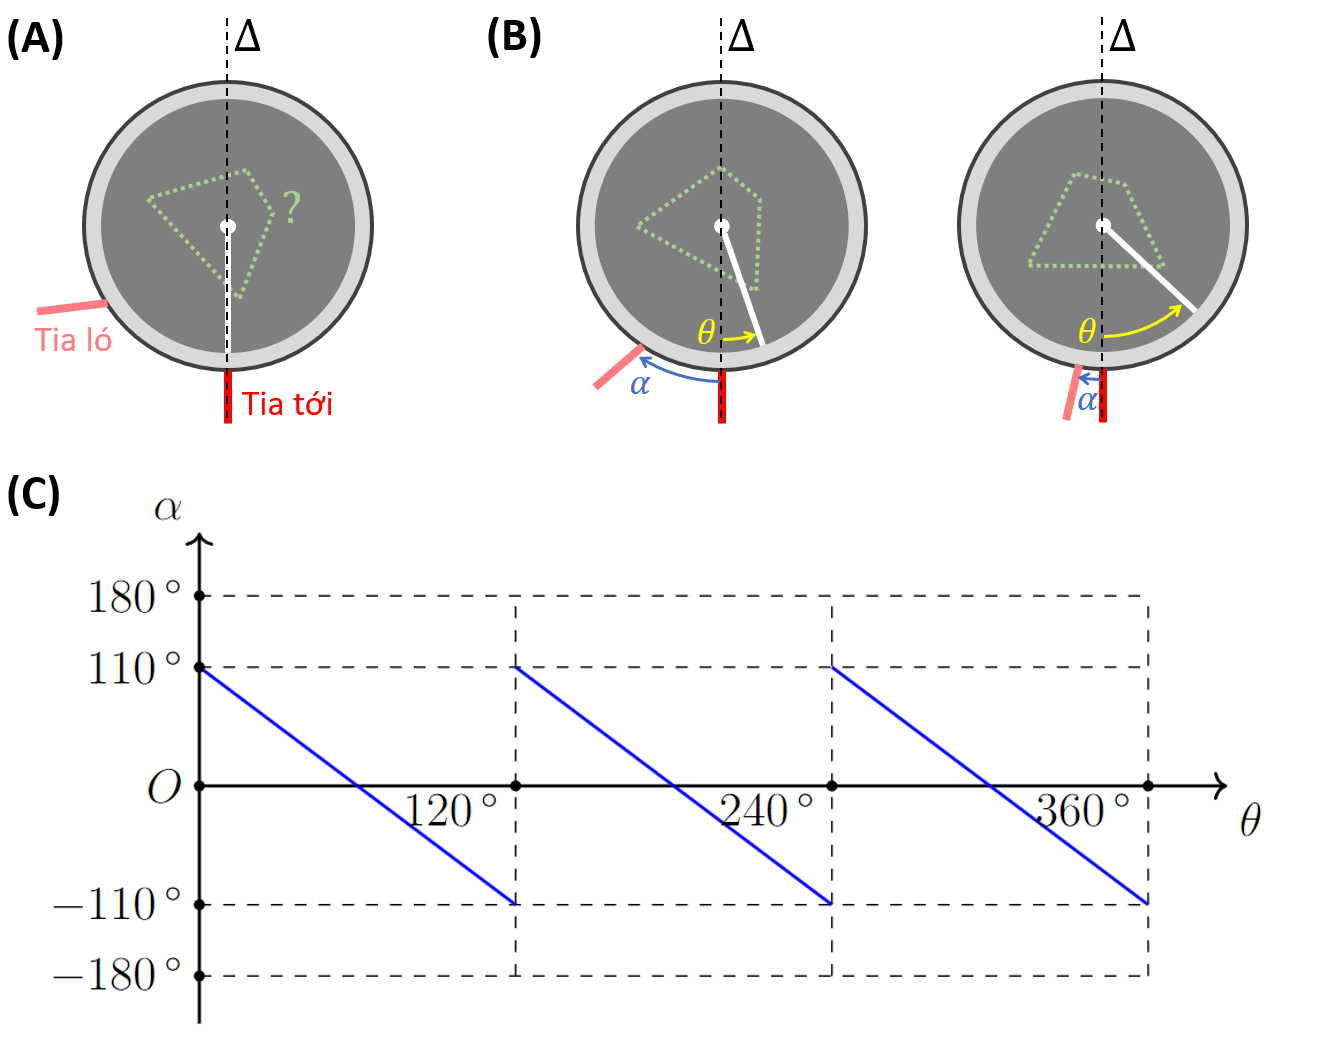
\includegraphics[width=0.8\textwidth,keepaspectratio]{Problem_4/Figs/P4.png}
\end{figure}

Biết $R=5cm$, và tâm khối hình học của lăng trụ trùng với trục xoay. Từ đồ thị $\alpha(\theta)$:
\begin{enumerate} [label=\roman*)]
        \item Tìm hình dạng và kích thước của vật.
        \item Ta thấy ba đoạn tách rời xuất hiện trên đồ thị, trông tương đối thẳng. Chúng có thực sự thẳng hay không? Tìm phương trình $\alpha(\theta)$ mô tả chúng.
\end{enumerate}



